\documentclass[border=10pt]{standalone}
\usepackage{amsmath,amssymb}
\usepackage[all]{xy}
\usepackage{tikz}
\usetikzlibrary{arrows,calc,positioning,fit, shapes.geometric}

\begin{document}
	\tikzstyle{operation} = [circle, text centered, minimum width=0.1cm, draw=black, font=\small]
	\tikzstyle{arrow} = [->, >=stealth]
	\tikzstyle{arrow_map} = [|->, >=stealth]
	\tikzstyle{oval} = [ellipse]
	
	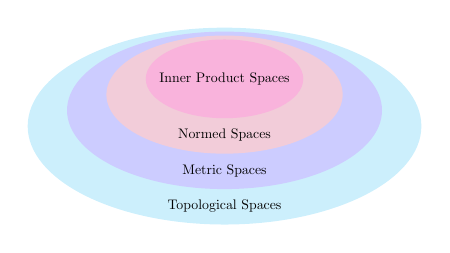
\begin{tikzpicture}
		\node[ellipse, fill=cyan!20, minimum width=5cm, minimum height=2.5cm] (topo) at (0,0) {};
		\node[ellipse, fill=blue!20, minimum width=4cm, minimum height=2cm] (metr) at(0,0.2) {};
		\node[ellipse, fill=purple!20, minimum width=3cm, minimum height=1.5cm] (norm) at(0, 0.4) {};
		\node[ellipse, fill=magenta!30, minimum width=2cm, minimum height=1cm] (inner) at(0, 0.6) {};
		
		\node[anchor=south, scale=0.5] (t) [above=0.1cm of topo.south] {Topological Spaces};
		\node[anchor=south, scale=0.5] (m) [above=0.1cm of metr.south] {Metric Spaces};
		\node[anchor=south, scale=0.5] (n) [above=0.1cm of norm.south] {Normed Spaces};
		\node[scale=0.5] (i) at (0, 0.6) {Inner Product Spaces};
	\end{tikzpicture}
\end{document}